% !TeX spellcheck = en_US

%TODO Leena

\begin{frame}{Snapshot Model}
\begin{itemize}
\item A model of conceptual neighborhood among topological relations between a line and a region.
\end{itemize}

		\begin{block}{Characteristics}
	\begin{itemize}
	
	\item No prior knowledge of the potential transformations that could lead from one configuration to the other. 
	\item Comparison on the basis of a pre-defined distance metric  
	\end{itemize}
	
		\end{block}
		
		\begin{block}{Differences of Intersections(\Empty = 0, \NotEmpty = 1)}
		\begin{figure}
		\begin{center}
			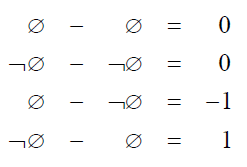
\includegraphics[width = 0.4\textwidth]{images/snapshotdiff.png}
		\end{center}
		\end{figure}
		\end{block}
	\end{frame}